\chapter{The Scope of the Work}
% TODO intro?
\section{The Current Situation}
The current way of acquiring new customers works as described in figure \ref{ScopeOfWork:Situation}.
\begin{figure}[ht]
  \centering
  % TODO neu in TikZ erstellen
  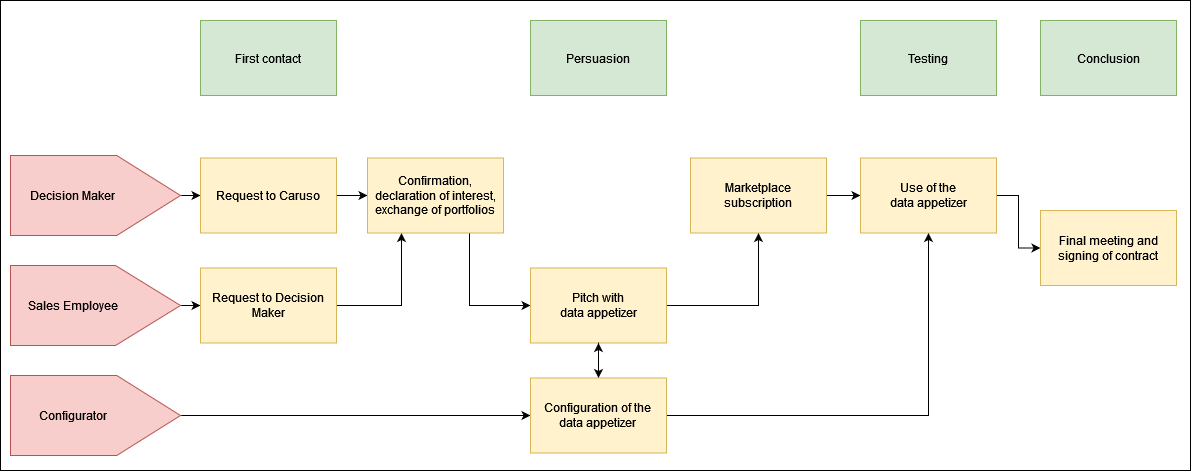
\includegraphics[width=20cm]{scope_of_the_work/current_situation.PNG}
  \caption{Stakeholders}
  \label{ScopeOfWork:Situation}
\end{figure}
Entry into a new contract currently requires three stakeholders: a decision maker, a Caruso sales employee and a Caruso configurator. The process can be split into four steps: first contact, persuasion, testing and conclusion. During first contact, the decision maker and sales employee enter into contact with each other. The sales employee gauges a decision makers interest in Caruso services or a decision maker becomes aware of Caruso through advertising, word of mouth or some other means.

After contact is established, the sales employee of Caruso holds a meeting with one or multiple decision makers. Here data items of publicly accessible cars , Caruso vehicles or dummy cars are presented. For this purpose, a manually created HTML or Excel report of aggregated vehicle data of past rides are created. These include data such as distance driven per day of the week for an entire fleet of cars.

After the sales pitch, the decision makers trusts and wants to use Caruso's services. They can then create an account in the Caruso Marketplace and receive the aggregated data shown during the presentation to look at for themselves. This data usually isn't live.

After the decision makers are convinced of the value of the data, a final meeting is held where any open questions can be discussed with the sales employee. Finally, a contract is entered by the two parties.

\section{The Context of the Work}
Figure \ref*{ScopeOfWork:ContextDiagram} shows the communication between the core target group, the Carvis and the neighbouring systems in the form of a context diagram.

% TODO in TikZ neu erstellen
% TODO Konfigurator unter Sales Employee
\begin{figure}[ht]
  \centering
  \includegraphics*[width=10cm]{./context_diagram.png}
  \caption{Context Diagram}
  \label{ScopeOfWork:ContextDiagram}
\end{figure}

The decision maker has access to both the Caruso Marketplace and Carvis. The access to the Marketplace is required as the decision maker needs to create an account and register vehicles before they can access Carvis.

The sales employee uses Carvis to present Caruso data to the decision maker. They are not allowed to access the decision makers data but can use placeholder cars publicly accessible in the Caruso Marketplace.

The configurator only needs access to Carvis in order to configure it for the sales employee.

Both systems get their data from the Caruso API which receives live data from the OEMs and standardises it.
% TODO ausformulieren?